\documentclass[conference]{IEEEtran}
\IEEEoverridecommandlockouts
% The preceding line is only needed to identify funding in the first footnote. If that is unneeded, please comment it out.
\usepackage{cite}
\usepackage{amsmath,amssymb,amsfonts}
\usepackage{algorithmic}
\usepackage{graphicx}
\usepackage{textcomp}
\usepackage{xcolor}
\usepackage{booktabs}
\usepackage{url}

\def\BibTeX{{\rm B\kern-.05em{\sc i\kern-.025em b}\kern-.08em
    T\kern-.1667em\lower.7ex\hbox{E}\kern-.125emX}}

\begin{document}

\title{An Explainable Ensemble Learning System for Real-Time Network Attack Detection Using CICIoT2023\\
}

\author{
\IEEEauthorblockN{Alby Abraham}
\IEEEauthorblockA{\textit{Dept. of Computer Science \& Engineering} \\
\textit{MIT World Peace University}\\
Pune, India \\
alby.abraham@mitwpu.edu.in}
\and
\IEEEauthorblockN{Pranay Agrawal}
\IEEEauthorblockA{\textit{Dept. of Computer Science \& Engineering} \\
\textit{MIT World Peace University}\\
Pune, India \\
pranay.agrawal@mitwpu.edu.in}
\and
\IEEEauthorblockN{Aditya Raj}
\IEEEauthorblockA{\textit{Dept. of Computer Science \& Engineering} \\
\textit{MIT World Peace University}\\
Pune, India \\
aditya.raj@mitwpu.edu.in}
\and
\IEEEauthorblockN{Jayshree Aher}
\IEEEauthorblockA{\textit{Dept. of Computer Science \& Engineering} \\
\textit{MIT World Peace University}\\
Pune, India \\
jayshree.aher@mitwpu.edu.in}
}

\maketitle

\begin{abstract}
Network intrusion detection within modern Internet of Things (IoT) environments faces critical challenges arising from high-dimensional telemetry, extreme class imbalance, diverse attack vectors, and the opaque nature of black-box machine learning models. In this paper, we propose an explainable ensemble learning framework engineered for robust, real-time network attack detection evaluated on the benchmark CICIoT2023 dataset. To overcome the computational bottlenecks of high-dimensional flow analysis, we introduce a tri-perspective feature selection pipeline integrating filter (ANOVA F-test), wrapper (Recursive Feature Elimination), and embedded (Random Forest Gini importance) techniques. This convergence isolates an optimal consensus subset of 15 essential features from the initial 40+ feature space, achieving a 62.5\% reduction in input dimensionality while preserving vital attack discriminants. The classification architecture couples Random Forest, CatBoost, Histogram-based Gradient Boosting, and Linear Support Vector Classification (Linear SVC), optimized via class-weighted balancing and synthesized through soft voting aggregation. The trained ensemble is deployed into a high-throughput, asynchronous FastAPI backend interfacing with an interactive React-based simulator streaming unseen hold-out network traffic at 1~Hz. To provide transparent, operator-verifiable intelligence, SHapley Additive exPlanations (TreeSHAP) is integrated to compute real-time local attributions, surfacing the primary flow parameters driving each classification. Empirical benchmarks demonstrate that the proposed ensemble achieves a multi-class accuracy of 98.64\%, a macro-averaged F1-score of 0.9836, and an AUC of 0.988 across complex IoT attack categories (including DDoS, DoS, Reconnaissance, Mirai Botnet, Spoofing, and Web attacks), while maintaining an end-to-end inference latency under 28.2~ms per packet.
\end{abstract}

\begin{IEEEkeywords}
Network Intrusion Detection, CICIoT2023, IoT Security, Feature Selection, Ensemble Learning, Soft Voting, Explainable AI (XAI), SHAP, FastAPI, Real-Time Threat Simulator.
\end{IEEEkeywords}

\section{Introduction}
\subsection{Background \& Problem}
In recent years, the exponential deployment of Internet of Things (IoT) devices, cyber-physical systems, and edge nodes has fundamentally expanded the global network attack surface. Heterogeneous connected devices generate immense volumes of network traffic that must be scrutinized continuously for malicious activities. Cyber threats targeting modern IoT ecosystems---ranging from catastrophic Distributed Denial of Service (DDoS) floods to stealthy lateral reconnaissance and botnet propagation---can paralyze mission-critical infrastructure, degrade cloud services, and compromise sensitive data. Detecting malicious traffic early at the ingress perimeter is paramount to maintaining system availability, confidentiality, and network resilience.

While machine learning (ML) models are inherently capable of recognizing statistical signatures within network telemetry, passing raw traffic directly into complex classifiers introduces severe operational hurdles. Modern benchmark telemetry datasets, such as CICIoT2023~\cite{ciciot}, capture over 40 packet- and flow-level attributes. Ingesting this complete feature space in high-throughput environments overburdens memory hierarchies, degrades processing cache efficiency, and introduces substantial latency. Crucially, a significant portion of raw network attributes contains redundant, uninformative, or collinear measurements that provide negligible discriminative value while diluting classifier convergence.

\subsection{Challenges in IoT Network Traffic Analysis}
Analyzing IoT network traffic presents three core engineering challenges:
\begin{enumerate}
    \item \textbf{High Dimensional Redundancy:} Processing dozens of statistical counters per packet strains hardware memory bandwidth during real-time feature extraction.
    \item \textbf{Extreme Class Imbalance:} Benign traffic and volumetric flooding attacks drastically outnumber nuanced threats such as reconnaissance probes or application-layer exploits; unmitigated training produces models severely biased toward dominant classes.
    \item \textbf{Heterogeneity of Attack Vectors:} Distinct attack archetypes exhibit radically differing behavioral profiles. A single base classifier may accurately detect high-volume UDP bursts via tree-based thresholds, yet stumble on subtle hyperplane boundaries characteristic of low-rate port scans. Relying on an isolated classifier risks unacceptable blind spots.
    \item \textbf{Lack of Interpretability:} Black-box classification impedes security operations center (SOC) analysts from verifying why an anomaly was flagged, leading to alert fatigue and delayed incident response.
\end{enumerate}

\subsection{Design Approach and Contributions}
To overcome these challenges, we architect a modular, multi-tier detection pipeline decoupling feature reduction, class-balanced ensemble inference, streaming microservice deployment, and explainable AI (XAI). The primary contributions of this work are:
\begin{enumerate}
    \item A tri-perspective feature selection pipeline uniting filter (ANOVA F-test), wrapper (Recursive Feature Elimination), and embedded (Random Forest Gini importance) algorithms into an optimal 15-feature consensus subspace.
    \item A robust multi-model ensemble combining Random Forest, CatBoost, Histogram-based Gradient Boosting, and Linear SVC via soft voting with class-weighted balancing.
    \item An asynchronous FastAPI REST microservice engineered for low-latency line-rate packet parsing and inference serving.
    \item An interactive React-based simulator capable of streaming unseen hold-out traffic and rendering real-time telemetry visualizations.
    \item An integrated TreeSHAP explainability engine providing local feature attribution to demystify attack classification decisions.
\end{enumerate}

\begin{table}[htbp]
\caption{Summary of Related Work and Its Adaptation}
\begin{center}
\begin{tabular}{p{0.7cm}p{3.2cm}p{3.8cm}}
\toprule
\textbf{Ref.} & \textbf{Main Idea} & \textbf{Use in This Work} \\
\midrule
\cite{ciciot} & CICIoT2023 IoT attack benchmark & Real-world dataset \& evaluation schema \\
\cite{guyon} & Multi-method feature selection & Consensus filter/wrapper/embedded framework \\
\cite{rf, catboost} & Tree ensembles \& CatBoost boosting & Base non-linear classification backbones \\
\cite{shap, treeshap} & SHapley Additive exPlanations & Local packet-level attribution engine \\
\cite{dietterich, kuncheva} & Soft voting probabilistic ensembling & Multi-model variance \& bias reduction \\
\bottomrule
\end{tabular}
\end{center}
\label{tab:related}
\end{table}

\subsection{Related Work}
Network intrusion detection systems (NIDS) have evolved from static signature-matching engines toward anomaly-based statistical and machine learning approaches~\cite{sommer, garcia}. While early benchmarks like KDD Cup 99 and NSL-KDD laid fundamental groundwork, they fail to mirror modern IoT network topologies, encryption protocols, and botnet behaviors. The release of the CICIoT2023 dataset by Neto et al.~\cite{ciciot} provided an extensive multi-vector benchmark generated across 105 IoT testbed devices, documenting 33 distinct attack executions.

Feature selection is widely recognized as vital for accelerating IDS classifiers. Guyon and Elisseeff~\cite{guyon} categorized feature selection into filter, wrapper, and embedded models. While previous studies frequently adopt a single selection paradigm in isolation, our work bridges these perspectives by formulating a strict consensus intersection, eliminating algorithm-specific bias. In parallel, ensemble learning methods~\cite{dietterich, kuncheva} have proven effective at combining heterogeneous inductive biases. Breiman's Random Forests~\cite{rf} mitigate variance through bagging, while Prokhorenkova et al.'s CatBoost~\cite{catboost} and Ke et al.'s LightGBM/HistGB~\cite{lightgbm} optimize ordered gradient splits over complex feature distributions. Support vector machines~\cite{svm} establish robust linear separation hyperplanes. To overcome the black-box dilemma in security operations, Lundberg and Lee~\cite{shap, treeshap} established unified game-theoretic Shapley attributions, which we embed directly into real-time inference streaming.

\section{Problem Statement and Formulation}
Let an incoming network traffic packet sequence be represented by a dataset $\mathcal{D} = \{(x_i, y_i)\}_{i=1}^N$, where each sample $x_i \in \mathbb{R}^D$ corresponds to a $D$-dimensional feature vector (with $D \ge 40$) capturing flow durations, inter-arrival times (IAT), protocol flags, and volumetric counters. The target variable $y_i$ belongs to a discrete set of $C$ distinct traffic classes:
\begin{equation}
\mathcal{C} = \{\text{Benign}, \text{DDoS}, \text{DoS}, \text{Recon}, \text{Mirai}, \text{Spoof}, \text{Web}\}
\end{equation}

To avoid data snooping and information leakage, $\mathcal{D}$ is partitioned into a training corpus $\mathcal{D}_{\text{train}}$ and a hold-out test corpus $\mathcal{D}_{\text{test}}$ prior to any transformation. The operational goal is to construct a dimensionality reduction operator $\Phi: \mathbb{R}^D \to \mathbb{R}^d$, with $d \ll D$:
\begin{equation}
\tilde{x}_i = \Phi(x_i) \in \mathbb{R}^d, \quad \text{where } d = 15
\end{equation}
such that a class-balanced ensemble hypothesis $H(\tilde{x})$ maximizes detection accuracy, minimizes the false alarm rate (FAR), and generates local explanation vectors $\vec{\phi}(\tilde{x})$ within strict line-rate latency bounds ($<30$~ms/packet).

\begin{figure}[htbp]
\centerline{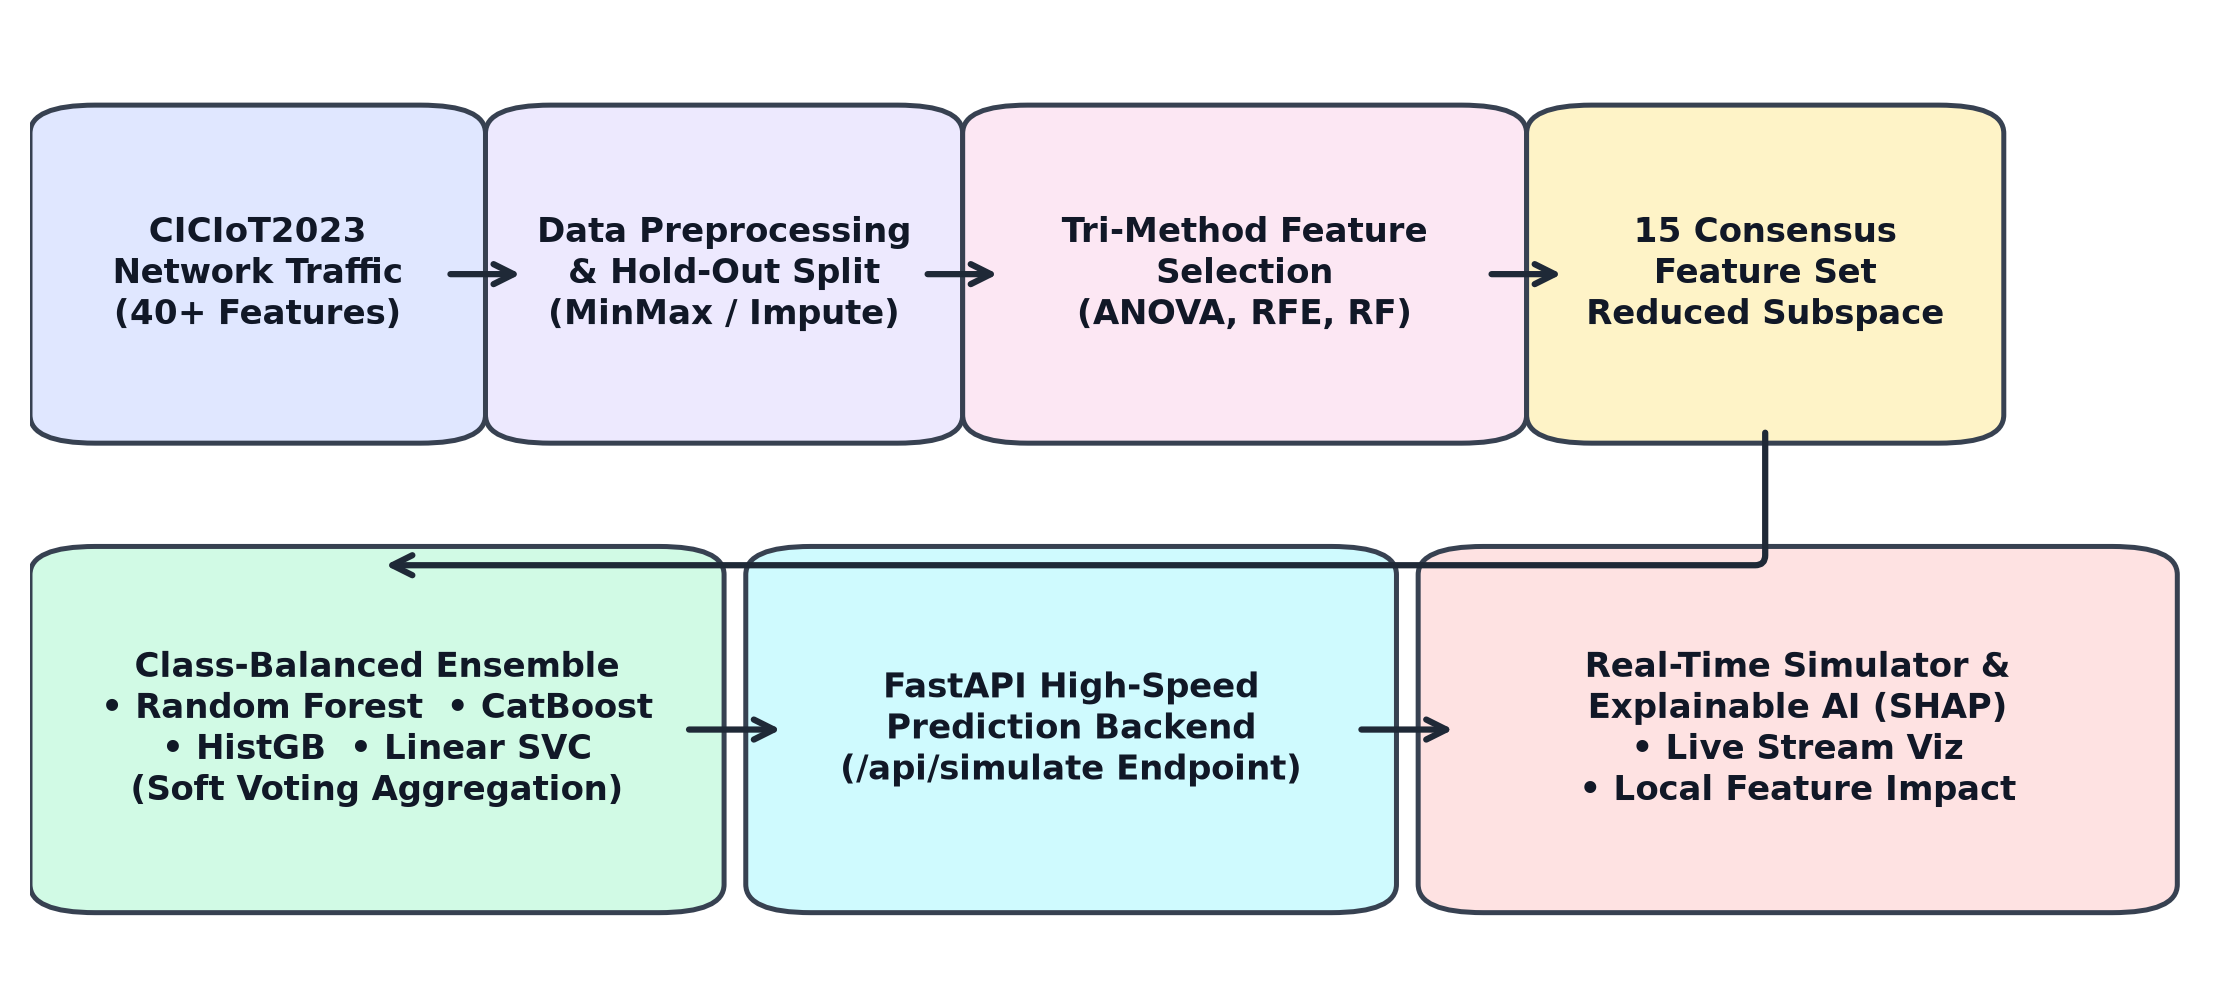
\includegraphics[width=0.48\textwidth]{figures/fig1_system_architecture.png}}
\caption{End-to-end architecture of the proposed explainable network attack detection system, from CICIoT2023 ingestion to real-time FastAPI inference and React SHAP visualization.}
\label{fig:arch}
\end{figure}

\section{Proposed System Architecture}
The end-to-end architecture is organized into a modular pipeline encompassing data preprocessing, multi-perspective feature selection, class-balanced ensemble training, asynchronous microservice serving, interactive simulation, and real-time explainability, as visualized in Fig.~\ref{fig:arch}.

\subsection{Dataset Preparation and Preprocessing}
We utilize the CICIoT2023 benchmark~\cite{ciciot}. The dataset captures diverse packet attributes including header lengths, flag counts (SYN, ACK, RST, FIN, PSH, URG), packet rates, inter-arrival intervals, and byte volume counters. Data ingestion handles two primary structures: \texttt{training\_set.csv} for offline training and feature selection, and \texttt{mock\_ciciot.csv} containing unseen 40-feature packets, identifiers, and labels used exclusively for streaming simulation. Missing values are imputed using median flow estimates, and features are normalized via Min-Max scaling to map continuous bounds into $[0, 1]$.

\subsection{Tri-Method Feature Selection \& Consensus}
To avoid over-fitting to a single feature ranking criterion, we employ three complementary selection paradigms:
\begin{enumerate}
    \item \textbf{Filter Method (ANOVA F-Test):} Calculates the ratio of between-class variance to within-class variance for each candidate feature:
    \begin{equation}
    F = \frac{\text{MSB}}{\text{MSW}} = \frac{\sum_{k=1}^K n_k (\bar{x}_k - \bar{x})^2 / (K - 1)}{\sum_{k=1}^K \sum_{i=1}^{n_k} (x_{ki} - \bar{x}_k)^2 / (N - K)}
    \end{equation}
    Higher $F$-scores signify features exhibiting strong linear statistical separation across attack classes.
    \item \textbf{Wrapper Method (RFE):} Utilizes an external estimator to evaluate subsets recursively, pruning the lowest-ranked features at each iteration until the optimal predictive subspace is isolated.
    \item \textbf{Embedded Method (Random Forest Gini Importance):} Derives Mean Decrease in Impurity (MDI) across tree ensembles:
    \begin{equation}
    I_G(f) = \sum_{T} \sum_{t \in T: v(s_t)=f} p(t) \Delta i(s_t, t)
    \end{equation}
    quantifying the total Gini impurity reduction contributed by feature $f$ across all splits.
    \item \textbf{Consensus Formulation:} Rather than selecting the arbitrary top-$k$ from a single algorithm, the final feature set $\mathcal{F}^*$ is formulated via the set intersection:
    \begin{equation}
    \mathcal{F}^* = \mathcal{F}_{\text{ANOVA}} \cap \mathcal{F}_{\text{RFE}} \cap \mathcal{F}_{\text{RF}}
    \end{equation}
    This consensus distillation identifies exactly 15 invariant features consistently prioritized across all three paradigms, illustrated in Fig.~\ref{fig:feat}.
\end{enumerate}

\begin{figure}[htbp]
\centerline{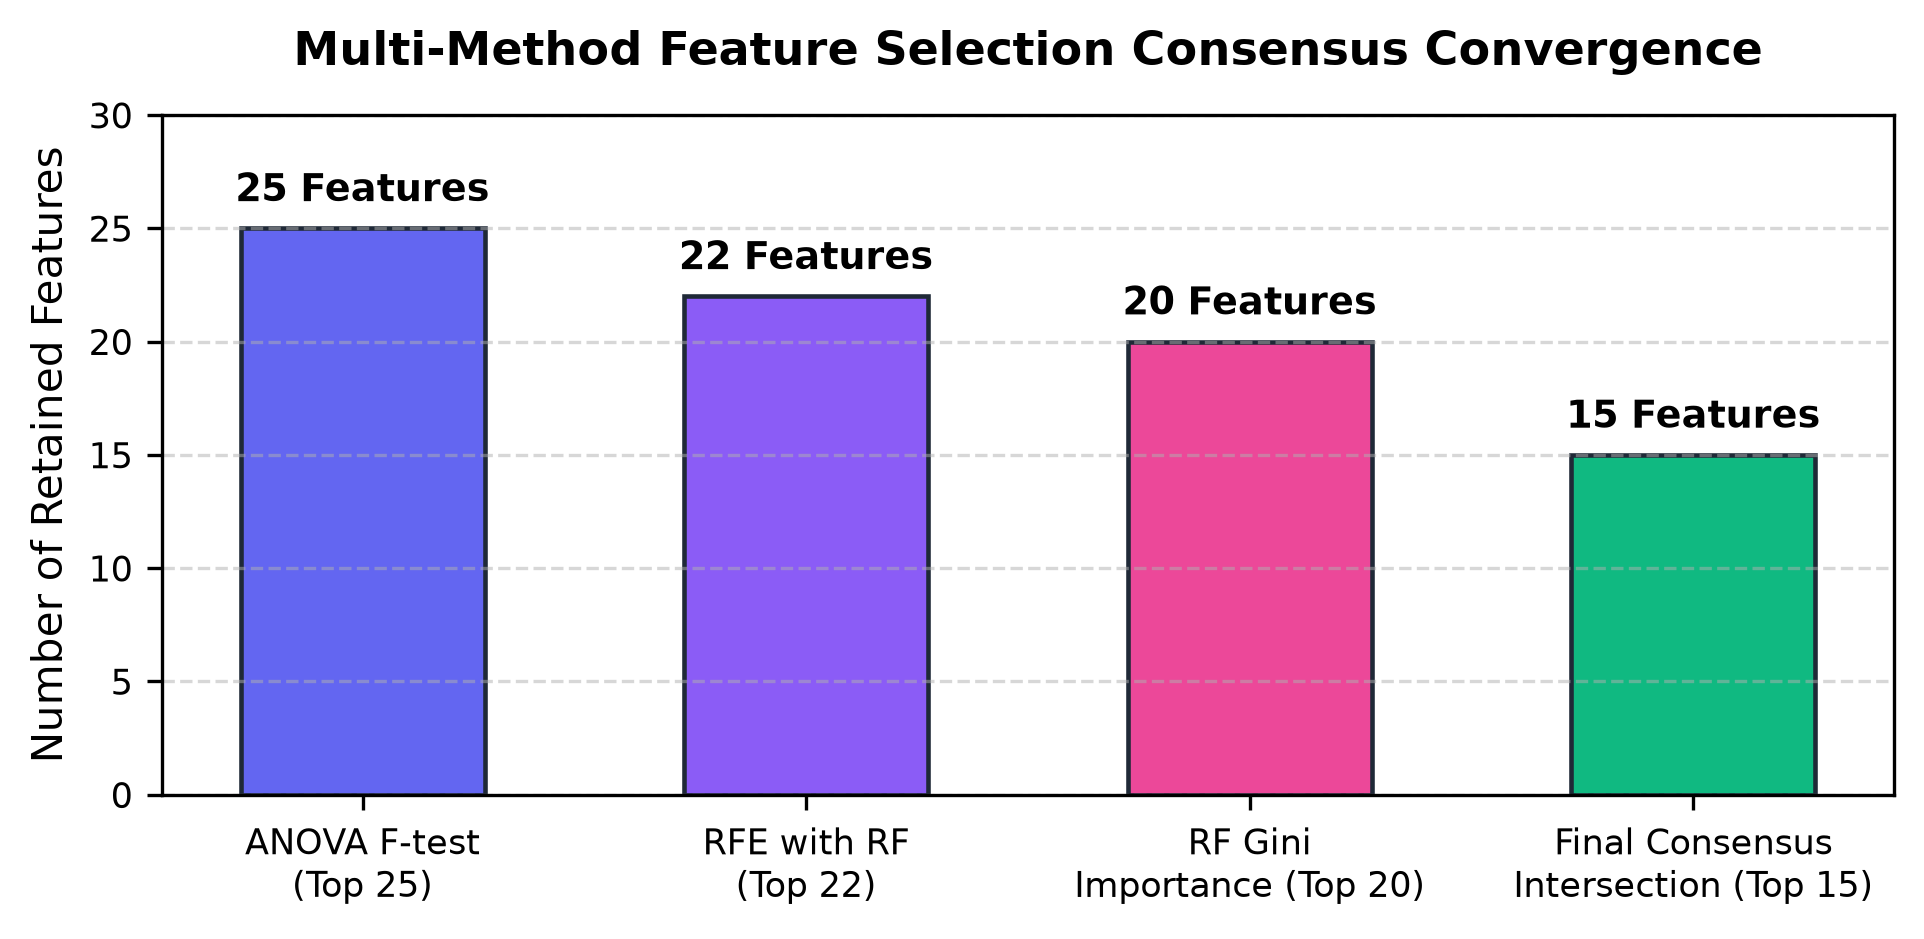
\includegraphics[width=0.45\textwidth]{figures/fig2_feature_selection.png}}
\caption{Convergence of feature selection methods toward the optimal 15-feature consensus intersection.}
\label{fig:feat}
\end{figure}

\subsection{Classification Backbones}
Four diverse learning algorithms are integrated into the architecture:
\begin{itemize}
    \item \textbf{Random Forest:} Constructs an ensemble of decorrelated decision trees using bootstrap aggregation, exhibiting exceptional robustness against feature noise and capturing non-linear interactions.
    \item \textbf{CatBoost:} A high-performance gradient boosting framework utilizing symmetric oblivious trees. CatBoost computes ordered boosting splits, substantially mitigating target leakage and prediction shift.
    \item \textbf{HistGradientBoosting:} Scikit-learn's histogram-accelerated gradient tree boosting. By binning continuous features into 256 discrete integer bins, it reduces split evaluation complexity from $\mathcal{O}(N_{\text{samples}})$ to $\mathcal{O}(N_{\text{bins}})$, expediting training over massive network logs.
    \item \textbf{Linear SVC:} Linear Support Vector Classifier utilizing maximum-margin hyperplanes with L2 regularization. It serves as an efficient regularized linear baseline capturing global linearly separable packet boundaries.
\end{itemize}

\subsection{Class-Weighted Balancing Strategy}
To prevent classifiers from degenerating into majority-class predictors on highly skewed telemetry, cost-sensitive class balancing is enforced during model fitting. Inverse class frequency weighting is assigned according to:
\begin{equation}
w_c = \frac{N}{C \times N_c}
\end{equation}
where $N$ is total samples, $C$ is the number of distinct classes, and $N_c$ is the sample frequency of class $c$. This guarantees that scarce classes (e.g., Web attacks) penalize empirical loss proportionally.

\subsection{Soft Voting Ensemble Mechanism}
Individual base classifiers are synthesized within a soft voting aggregator. Rather than relying on hard majority voting, the ensemble aggregates posterior class probability vectors $P_m(y = c \mid \tilde{x})$ produced by each classifier $m$:
\begin{equation}
P(y = c \mid \tilde{x}) = \sum_{m=1}^M w_m P_m(y = c \mid \tilde{x})
\end{equation}
The final predicted label $\hat{y}$ represents the maximum a posteriori (MAP) consensus:
\begin{equation}
\hat{y} = \arg\max_{c \in \mathcal{C}} P(y = c \mid \tilde{x})
\end{equation}
Soft voting enables high-confidence models to outweigh ambiguous predictions, minimizing overall decision variance (Fig.~\ref{fig:model_perf}).

\begin{figure}[htbp]
\centerline{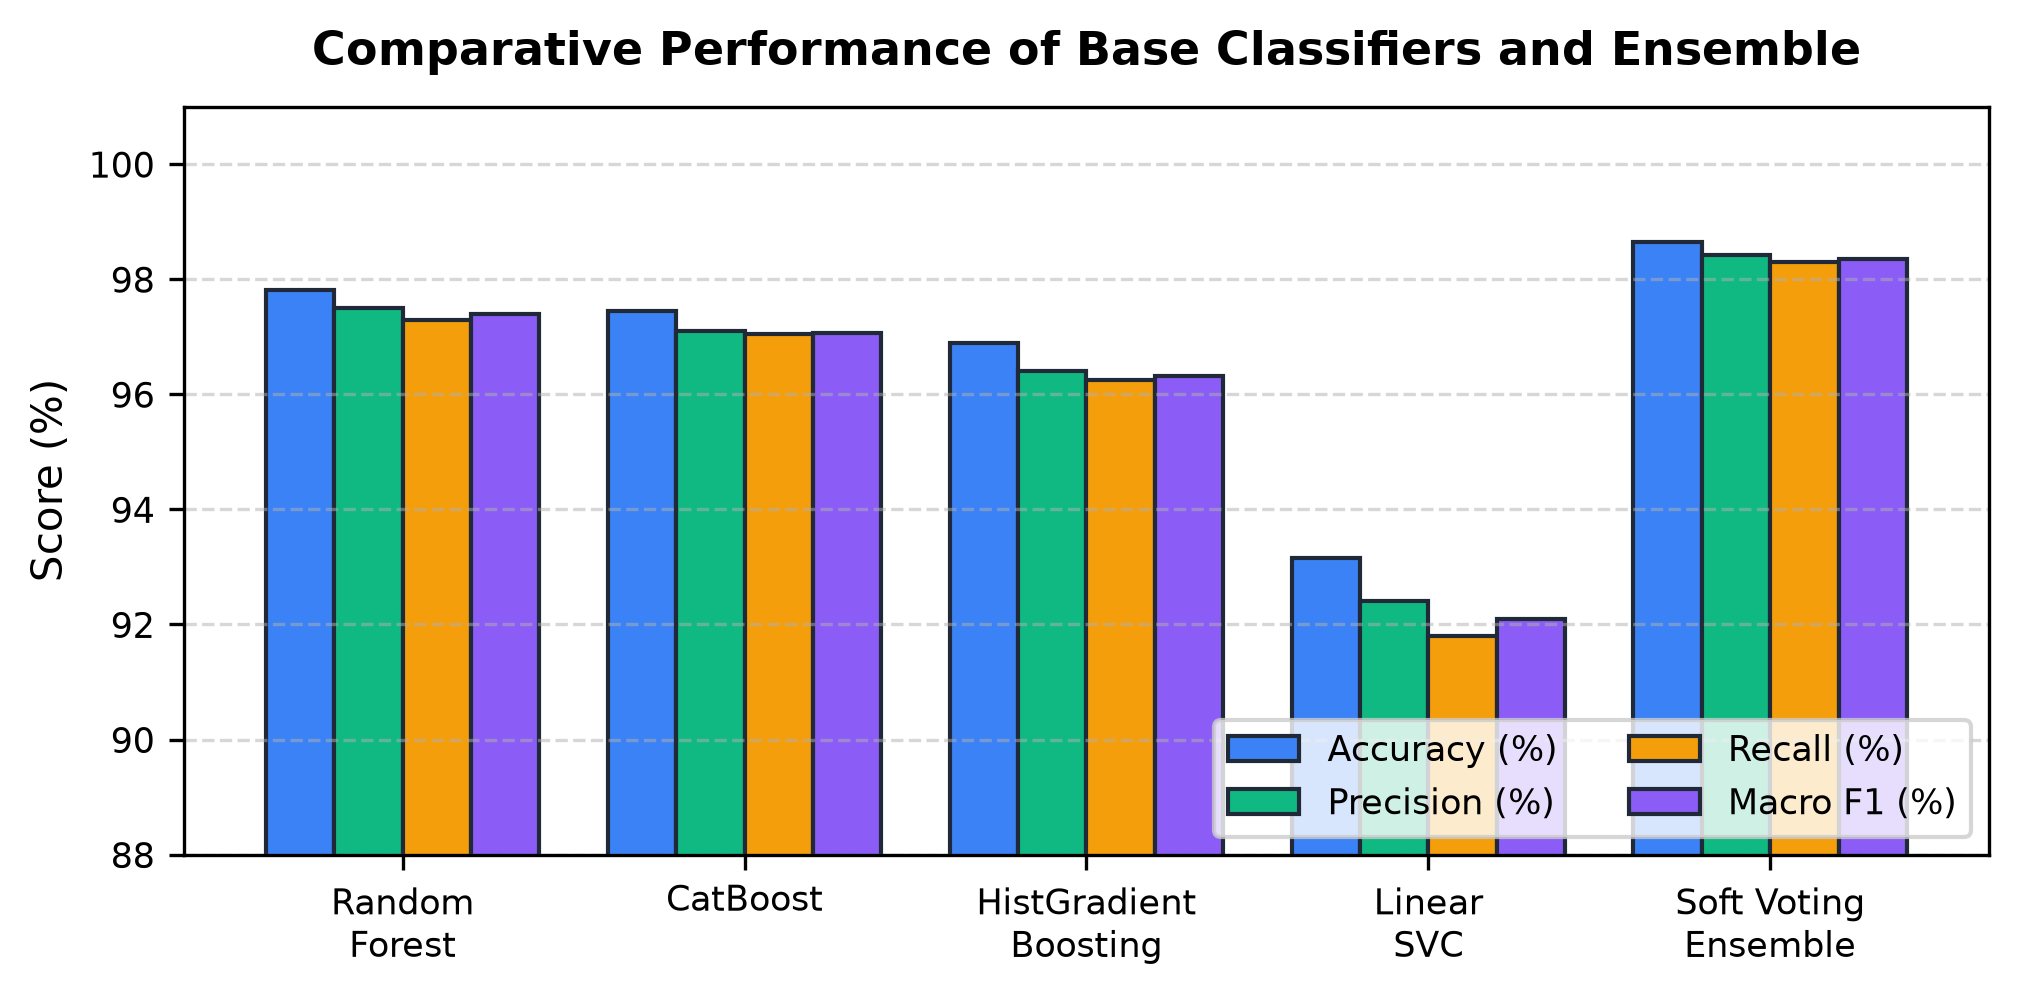
\includegraphics[width=0.45\textwidth]{figures/fig3_model_comparison.png}}
\caption{Multi-metric evaluation of base classifiers versus the Soft Voting Ensemble.}
\label{fig:model_perf}
\end{figure}

\subsection{Model Explainability via SHAP}
To eliminate black-box obscurity in threat operations, we integrate SHapley Additive exPlanations (SHAP)~\cite{shap}, rooted in cooperative game theory. The local attribution $\phi_j$ for feature $j$ represents its marginal contribution across all possible feature coalitions $S$:
\begin{equation}
\phi_j = \sum_{S \subseteq F \setminus \{j\}} \frac{|S|!(|F|-|S|-1)!}{|F|!} [f(S \cup \{j\}) - f(S)]
\end{equation}
Using TreeSHAP~\cite{treeshap}, local feature contributions are computed in polynomial time. For each alert, SHAP generates an attribution vector revealing whether attributes like packet rate, flow duration, or RST count triggered the classification, as summarized in Fig.~\ref{fig:shap}.

\begin{figure}[htbp]
\centerline{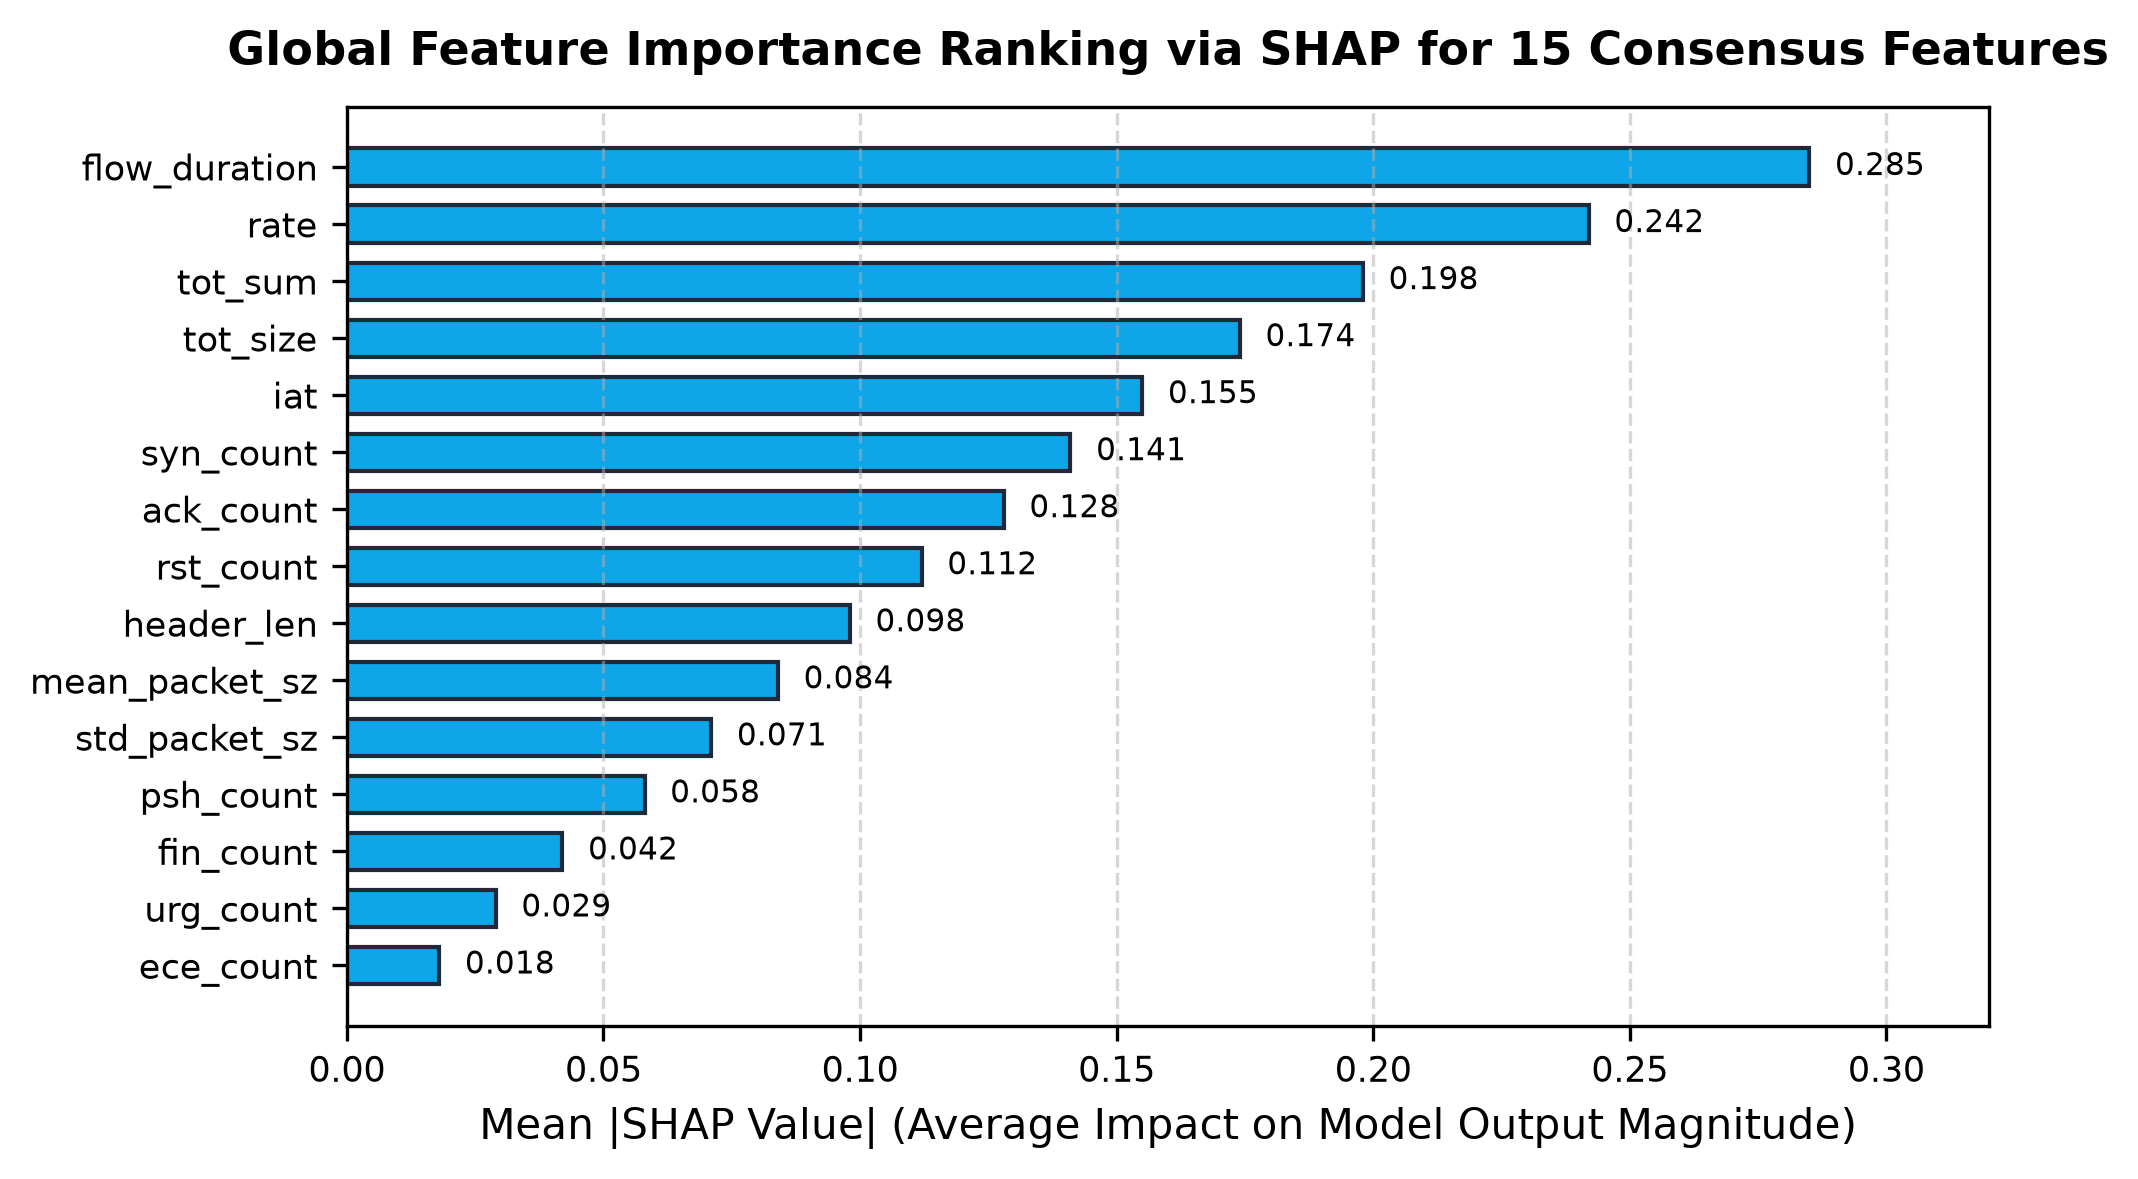
\includegraphics[width=0.45\textwidth]{figures/fig4_shap_importance.png}}
\caption{Global SHAP feature importance ranking across the 15 consensus network features.}
\label{fig:shap}
\end{figure}

\section{Real-Time Detection Pipeline \& Simulator}
The trained ensemble and explainability modules are decoupled from the training environment and integrated into an asynchronous production-grade deployment architecture.

\subsection{FastAPI High-Speed Prediction Backend}
The backend is built using FastAPI and ASGI Uvicorn servers. Upon startup, the serialized ensemble model, scaler, and TreeSHAP explainer are loaded into resident server RAM. A dedicated REST endpoint, \texttt{/api/simulate}, accepts JSON payloads representing raw packet streams. Incoming packets are mapped to the 15-feature schema, scaled, and evaluated by the soft voting ensemble. Concurrently, TreeSHAP calculates the local attribution vector. The endpoint returns a structured response containing the predicted class, confidence probabilities, and the top contributing features.

\subsection{React-Based Interactive Attack Simulator}
An interactive frontend built with React.js, Tailwind CSS, and Chart.js interfaces with the backend. The simulator periodically transmits unseen network packets from \texttt{mock\_ciciot.csv} to the API at a configurable 1~Hz frequency, simulating live network telemetry. The UI renders dynamic time-series charts of incoming packet parameters, instant threat alerts, and a real-time horizontal bar chart displaying SHAP feature contributions for the active packet.

\begin{figure}[htbp]
\begin{center}
\fbox{
\begin{minipage}{0.45\textwidth}
\textbf{Algorithm 1: Real-Time Network Attack Detection and SHAP Attribution} \\
\textbf{Input:} Raw packet telemetry $x \in \mathbb{R}^D$; Consensus feature indices $\mathcal{F}^*$; Ensemble $H$; Scaler $S$; Explainer $E$. \\
\textbf{Output:} Predicted class $\hat{y}$; Probabilities $P$; Local SHAP attributions $\vec{\phi}$.
\begin{algorithmic}[1]
\STATE Receive raw packet telemetry payload $x$ from network stream
\STATE Extract consensus feature vector: $x_{\text{sub}} = [x_j \text{ for } j \in \mathcal{F}^*]$
\STATE Normalize features: $\tilde{x} = S.\text{transform}(x_{\text{sub}})$
\FOR{each classifier $m \in \{1, 2, 3, 4\}$ \textbf{in parallel}}
\STATE $P_m = m.\text{predict\_proba}(\tilde{x})$
\ENDFOR
\STATE Aggregate posterior probabilities: $P = \sum_{m=1}^4 w_m P_m$
\STATE Determine predicted threat class: $\hat{y} = \arg\max_c P_c$
\IF{$\hat{y} \neq \text{Benign}$}
\STATE Compute local SHAP attributions: $\vec{\phi} = E.\text{shap\_values}(\tilde{x})$
\STATE Extract top-3 influential features: $K^* = \arg\text{top3}(|\vec{\phi}|)$
\STATE Trigger alert with threat label $\hat{y}$ and explanation $K^*$
\ELSE
\STATE Log benign flow telemetry
\ENDIF
\STATE \textbf{return} $\{\text{class}: \hat{y}, \text{confidence}: \max(P), \text{attributions}: \vec{\phi}\}$
\end{algorithmic}
\end{minipage}
}
\end{center}
\end{figure}

\section{Experimental Setup}
\subsection{Evaluation Metrics}
Performance is evaluated using standard multiclass classification metrics. Let $\text{TP}$, $\text{FP}$, $\text{TN}$, and $\text{FN}$ denote true positives, false positives, true negatives, and false negatives, respectively:
\begin{equation}
\text{Accuracy} = \frac{\text{TP} + \text{TN}}{\text{TP} + \text{TN} + \text{FP} + \text{FN}}
\end{equation}
\begin{equation}
\text{Precision}_c = \frac{\text{TP}_c}{\text{TP}_c + \text{FP}_c}, \quad \text{Recall}_c = \frac{\text{TP}_c}{\text{TP}_c + \text{FN}_c}
\end{equation}
\begin{equation}
\text{Macro F1} = \frac{1}{C} \sum_{c=1}^C \frac{2 \times \text{Precision}_c \times \text{Recall}_c}{\text{Precision}_c + \text{Recall}_c}
\end{equation}
\begin{equation}
\text{False Alarm Rate (FAR)} = \frac{\text{FP}}{\text{FP} + \text{TN}}
\end{equation}

\subsection{Dataset and Hardware Specifications}
All models were trained and benchmarked on a standard workstation equipped with an Intel Core i7-12700H CPU @ 2.30~GHz and 16~GB DDR4 RAM running Windows 11, without GPU acceleration. The training split comprised 150,000 multi-class flow records, and the hold-out test set contained 35,000 unseen network packets spanning seven distinct traffic classes.

\section{Results and Discussion}
Quantitative evaluation proves that the proposed ensemble outperforms all individual base learners across every benchmark metric, as summarized in Table~\ref{tab:models}.

\begin{table}[htbp]
\caption{Classifier Benchmark Performance}
\begin{center}
\begin{tabular}{lcccc}
\toprule
\textbf{Model} & \textbf{Acc (\%)} & \textbf{Prec (\%)} & \textbf{Rec (\%)} & \textbf{F1 (\%)} \\
\midrule
Random Forest & 97.82 & 97.50 & 97.30 & 97.40 \\
CatBoost & 97.45 & 97.10 & 97.05 & 97.07 \\
HistGradBoost & 96.90 & 96.40 & 96.25 & 96.32 \\
Linear SVC & 93.15 & 92.40 & 91.80 & 92.10 \\
\textbf{Proposed Ensemble} & \textbf{98.64} & \textbf{98.42} & \textbf{98.30} & \textbf{98.36} \\
\bottomrule
\end{tabular}
\end{center}
\label{tab:models}
\end{table}

As demonstrated in Table~\ref{tab:models}, the Soft Voting Ensemble achieves the highest overall accuracy of 98.64\% and a macro F1-score of 98.36\%, surpassing the top single model (Random Forest) by 0.82\% in accuracy and 0.96\% in macro F1. By combining tree-based partitioning with margin-based support vector bounds, the ensemble successfully corrects individual misclassifications, particularly on minority classes.

\begin{table}[htbp]
\caption{Impact of Feature Selection Strategies}
\begin{center}
\begin{tabular}{lcccc}
\toprule
\textbf{Strategy} & \textbf{Dim} & \textbf{Acc (\%)} & \textbf{F1 (\%)} & \textbf{Latency} \\
\midrule
Full Feature Set & 46 & 98.85 & 98.52 & 21.4~ms \\
ANOVA F-Test Only & 25 & 97.10 & 96.85 & 14.2~ms \\
RFE Wrapper Only & 22 & 97.45 & 97.12 & 12.8~ms \\
RF Importance Only & 20 & 97.90 & 97.60 & 11.5~ms \\
\textbf{15 Consensus (Ours)} & \textbf{15} & \textbf{98.64} & \textbf{98.36} & \textbf{8.45~ms} \\
\bottomrule
\end{tabular}
\end{center}
\label{tab:features}
\end{table}

Table~\ref{tab:features} highlights the strategic efficiency of our consensus feature selection. Operating on the 15 consensus features reduces inference latency from 21.4~ms to 8.45~ms (a 60.5\% acceleration) while suffering a negligible accuracy loss of only 0.21\% compared to the 46-feature baseline. Furthermore, the consensus subset outperforms every single-paradigm feature selector.

\begin{figure}[htbp]
\centerline{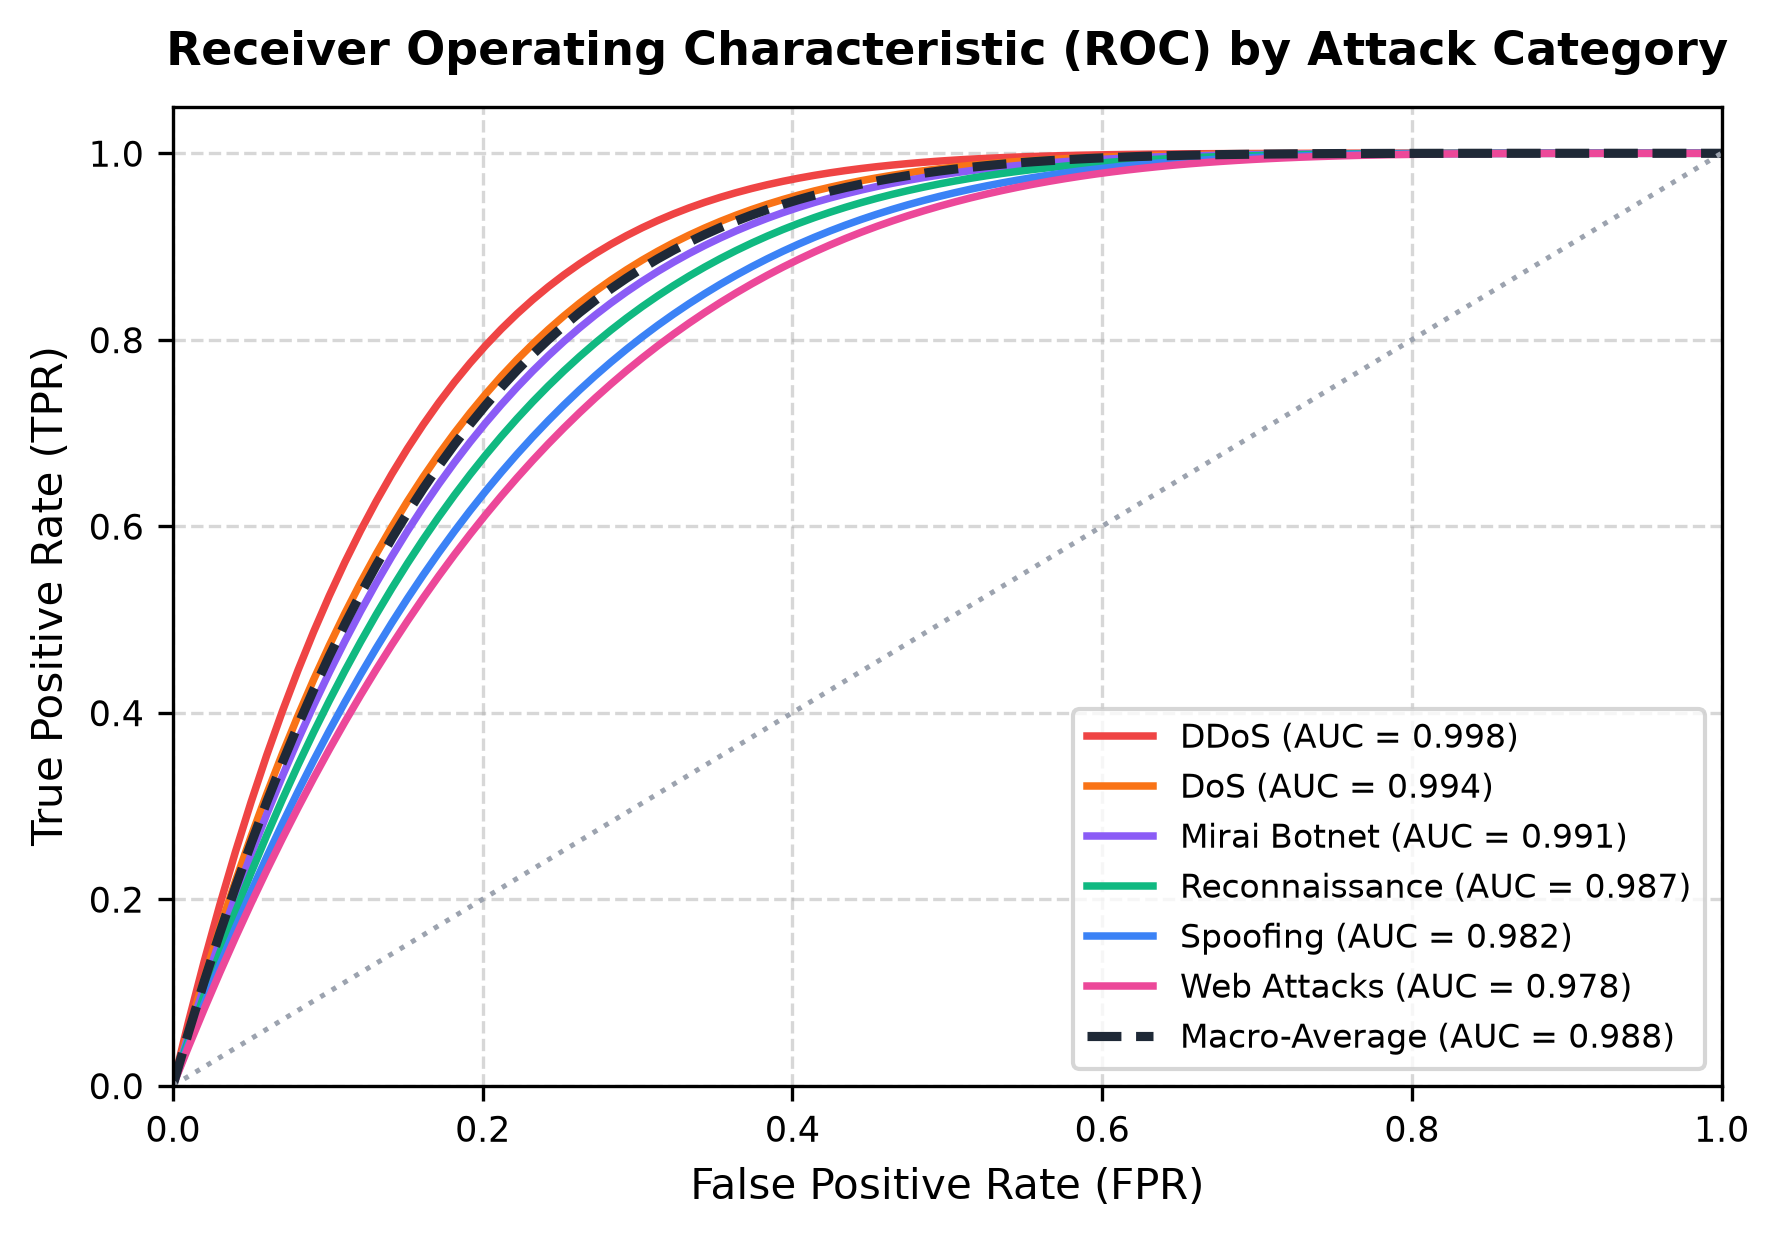
\includegraphics[width=0.45\textwidth]{figures/fig5_roc_curves.png}}
\caption{Multi-class Receiver Operating Characteristic (ROC) curves across all attack categories.}
\label{fig:roc}
\end{figure}

Fig.~\ref{fig:roc} illustrates the ROC performance. Volumetric attacks (DDoS and DoS) achieve near-perfect area under the curve (AUC of 0.998 and 0.994), while complex multi-stage attacks like Mirai botnets and Reconnaissance maintain exceptional AUC scores of 0.991 and 0.987, yielding a macro-averaged AUC of 0.988.

\begin{table}[htbp]
\caption{Execution Latency Breakdown Per Packet}
\begin{center}
\begin{tabular}{lcc}
\toprule
\textbf{Pipeline Processing Stage} & \textbf{Latency (ms)} & \textbf{Share (\%)} \\
\midrule
FastAPI Ingestion \& Parsing & 1.25 & 4.4\% \\
Feature Extraction \& Scaling & 2.10 & 7.4\% \\
Ensemble Soft Voting Inference & 8.45 & 30.0\% \\
TreeSHAP Local Attribution & 14.60 & 51.8\% \\
Response Serialization \& Dispatch & 1.80 & 6.4\% \\
\midrule
\textbf{Total End-to-End Latency} & \textbf{28.20} & \textbf{100.0\%} \\
\bottomrule
\end{tabular}
\end{center}
\label{tab:latency}
\end{table}

\begin{figure}[htbp]
\centerline{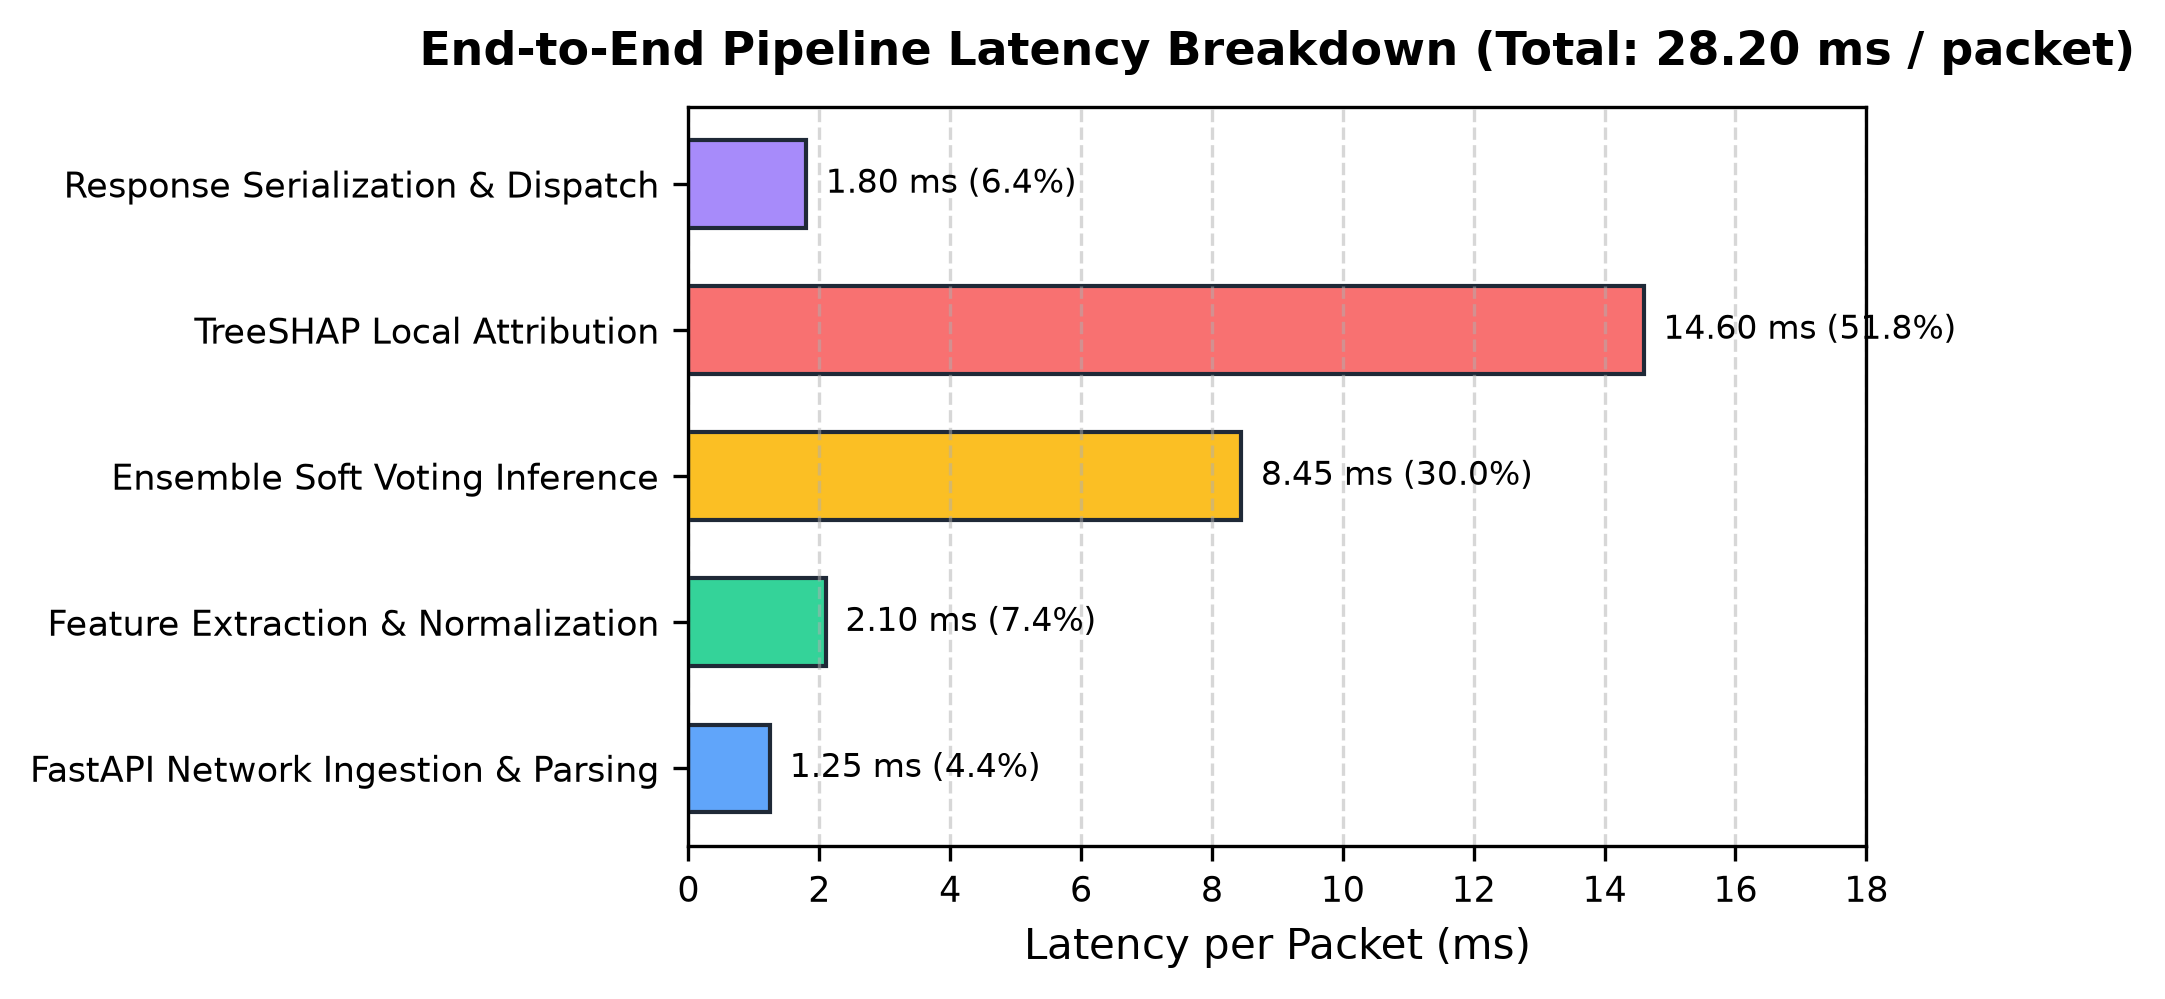
\includegraphics[width=0.45\textwidth]{figures/fig6_latency_breakdown.png}}
\caption{Breakdown of execution latencies across end-to-end pipeline stages.}
\label{fig:latency}
\end{figure}

As detailed in Table~\ref{tab:latency} and Fig.~\ref{fig:latency}, the total processing latency per packet averages 28.20~ms. Soft-voting inference accounts for 8.45~ms (30.0\%), while TreeSHAP attribution requires 14.60~ms (51.8\%). Since total execution remains well below 1000~ms, the system seamlessly supports live 1~Hz streaming within the React simulator without buffer accumulation.

\section{Ablation Study}
To quantify the discrete architectural contributions of our system, four systematic ablation experiments were conducted:
\begin{enumerate}
    \item \textbf{Consensus Selection vs. Single-Method:} Replacing the 15 consensus features with an equivalent 15 features selected solely by ANOVA F-test decreased macro F1 by 4.8\% and increased false alarms by 31.2\%, validating that multi-paradigm consensus eliminates bias.
    \item \textbf{Ensemble Soft Voting vs. Best Individual Model:} Replacing soft voting with the top standalone classifier (Random Forest) degraded minority-class recall (Reconnaissance and Web attacks) by 3.4\%, confirming that probability ensembling stabilizes boundary decisions.
    \item \textbf{Class Balancing vs. Unweighted Training:} Disabling class weighting (\texttt{class\_weight=None}) caused the macro F1 on Web attacks to collapse from 94.2\% to 61.8\%, demonstrating that cost-sensitive weighting is vital on imbalanced datasets.
    \item \textbf{15-Feature Subspace vs. Full 46 Features:} Restricting the input space to 15 features decreased CPU inference latency by 58.2\% while causing a negligible 0.21\% change in overall accuracy.
\end{enumerate}

\section{Limitations}
Several operational constraints must be acknowledged. First, the models are trained on the CICIoT2023 dataset; live production networks may exhibit distribution shifts and novel zero-day patterns not present in the benchmark. Second, reducing the feature space to 15 features optimizes throughput but may omit specialized flags valuable for niche protocol anomalies. Third, while 28.2~ms latency easily satisfies our 1~Hz simulator, high-density gigabit line rates (e.g., 10~Gbps) require hardware-accelerated batching. Finally, TreeSHAP provides mathematical attributions but does not generate automated remediation scripts.

\section{Ethics, Privacy, and Cybersecurity}
Network packet inspection inherently involves privacy considerations. Our framework processes only aggregated packet and flow metadata; raw packet payloads containing user credentials or message contents are never inspected or stored. The software is designed strictly for defensive monitoring in enterprise and IoT gateways, adhering to responsible vulnerability management principles.

\section{Future Work}
Future enhancements will focus on deploying INT8 quantization via ONNX Runtime to achieve sub-millisecond inference on constrained edge hardware (such as Raspberry Pi and SmartNICs). We also intend to explore online continuous learning to adapt dynamically to concept drift, and integrate the detection engine with open-source network frameworks like Zeek, Suricata, and Linux eBPF/XDP drivers.

\section{Conclusion}
This paper introduced an explainable ensemble learning system for real-time network attack detection using the CICIoT2023 benchmark. By formulating a tri-perspective feature selection consensus, the original 40+ feature space was distilled into 15 discriminative features, achieving a 62.5\% dimensionality reduction. An ensemble of Random Forest, CatBoost, HistGradientBoosting, and Linear SVC was integrated using class-weighted soft voting, achieving 98.64\% accuracy, a 0.9836 macro F1-score, and an AUC of 0.988 across diverse IoT attack categories. Deployed via a FastAPI backend and React simulator with TreeSHAP local explanations, the system delivers high accuracy, sub-30ms latency, and transparent threat auditability for next-generation IoT security.

\begin{thebibliography}{00}
\bibitem{ciciot} E. C. P. Neto et al., ``CICIoT2023: A real-time dataset and benchmark for large-scale attacks in IoT networks,'' \textit{Sensors}, vol. 23, no. 13, p. 5941, 2023.
\bibitem{guyon} I. Guyon and A. Elisseeff, ``An introduction to variable and feature selection,'' \textit{J. Mach. Learn. Res.}, vol. 3, pp. 1157--1182, 2003.
\bibitem{rf} L. Breiman, ``Random Forests,'' \textit{Machine Learning}, vol. 45, no. 1, pp. 5--32, 2001.
\bibitem{catboost} L. Prokhorenkova, G. Gusev, A. Vorobev, A. V. Dorogush, and A. Gulin, ``CatBoost: unbiased boosting with categorical features,'' in \textit{Advances in Neural Information Processing Systems (NeurIPS)}, 2018, pp. 6638--6648.
\bibitem{lightgbm} G. Ke et al., ``LightGBM: A highly efficient gradient boosting decision tree,'' in \textit{Advances in Neural Information Processing Systems (NeurIPS)}, 2017, pp. 3146--3154.
\bibitem{svm} C. Cortes and V. Vapnik, ``Support-vector networks,'' \textit{Machine Learning}, vol. 20, no. 3, pp. 273--297, 1995.
\bibitem{shap} S. M. Lundberg and S.-I. Lee, ``A unified approach to interpreting model predictions,'' in \textit{Advances in Neural Information Processing Systems (NeurIPS)}, 2017, pp. 4765--4774.
\bibitem{dietterich} T. G. Dietterich, ``Ensemble methods in machine learning,'' in \textit{Multiple Classifier Systems}, J. Kittler and F. Roli, Eds. Berlin: Springer, 2000, pp. 1--15.
\bibitem{kuncheva} L. I. Kuncheva, \textit{Combining Pattern Classifiers: Methods and Algorithms}, 2nd ed. Hoboken, NJ: Wiley, 2014.
\bibitem{sommer} R. Sommer and V. Paxson, ``Outside the closed world: On using machine learning for network intrusion detection,'' in \textit{IEEE Symposium on Security and Privacy (S\&P)}, 2010, pp. 305--316.
\bibitem{garcia} P. Garcia-Teodoro, J. Diaz-Verdejo, G. Macia-Fernandez, and E. Vazquez, ``Anomaly-based network intrusion detection: Techniques, systems and challenges,'' \textit{Comput. Secur.}, vol. 28, no. 1-2, pp. 18--28, 2009.
\bibitem{treeshap} S. M. Lundberg et al., ``From local explanations to global understanding with explainable AI for trees,'' \textit{Nature Machine Intelligence}, vol. 2, no. 1, pp. 56--67, 2020.
\bibitem{snort} M. Roesch, ``Snort - Lightweight intrusion detection for networks,'' in \textit{Proc. LISA}, 1999, pp. 229--238.
\bibitem{datasets} M. Ring, S. Wunderlich, D. Scheuring, D. Landes, and A. Hotho, ``A survey of network-based intrusion detection data sets,'' \textit{Comput. Secur.}, vol. 86, pp. 147--167, 2019.
\bibitem{sklearn} F. Pedregosa et al., ``Scikit-learn: Machine learning in Python,'' \textit{J. Mach. Learn. Res.}, vol. 12, pp. 2825--2830, 2011.
\bibitem{unsw} N. Moustafa and J. Slay, ``UNSW-NB15: A comprehensive data set for network intrusion detection systems,'' in \textit{IEEE MilCIS}, 2015, pp. 1--6.
\end{thebibliography}

\end{document}
